\documentclass[10pt,a4paper]{article}
\usepackage[utf8]{inputenc}
\usepackage[brazil]{babel}
\usepackage{amsmath}
\usepackage{amsfonts}
\usepackage{amssymb}
\usepackage{graphicx}
\usepackage{enumerate}
\usepackage{indentfirst}

\author{Myke Albuquerque Pinto de Oliveira}
\title{\Huge Atividade a Distância 1 \\ 
	Aplicações das Integrais Múltiplas}

\newcommand{\sen}{\hspace{2pt}\textrm{sen}}
\newcommand{\tg}{\hspace{2pt}\textrm{tg}}

\begin{document}
	
	\maketitle
	\newpage
	
	\section*{Questão 1}
	
	Dada a integral dupla $ \int_{0}^{\frac{\pi}{6}} \int_{0}^{\frac{\pi}{3}} x \sen (x + y) dy dx $, desenvolva os seguites itens.
	
	\begin{enumerate}[a]
		\item Descreva graficamente a região de integração.
		\item Calcule a integral dada usando a ordem de integração que você achar mais conveniente.
	\end{enumerate}
	
	(Valor da questão: 1,0)
	
	\begin{figure}[h]
		\centering
		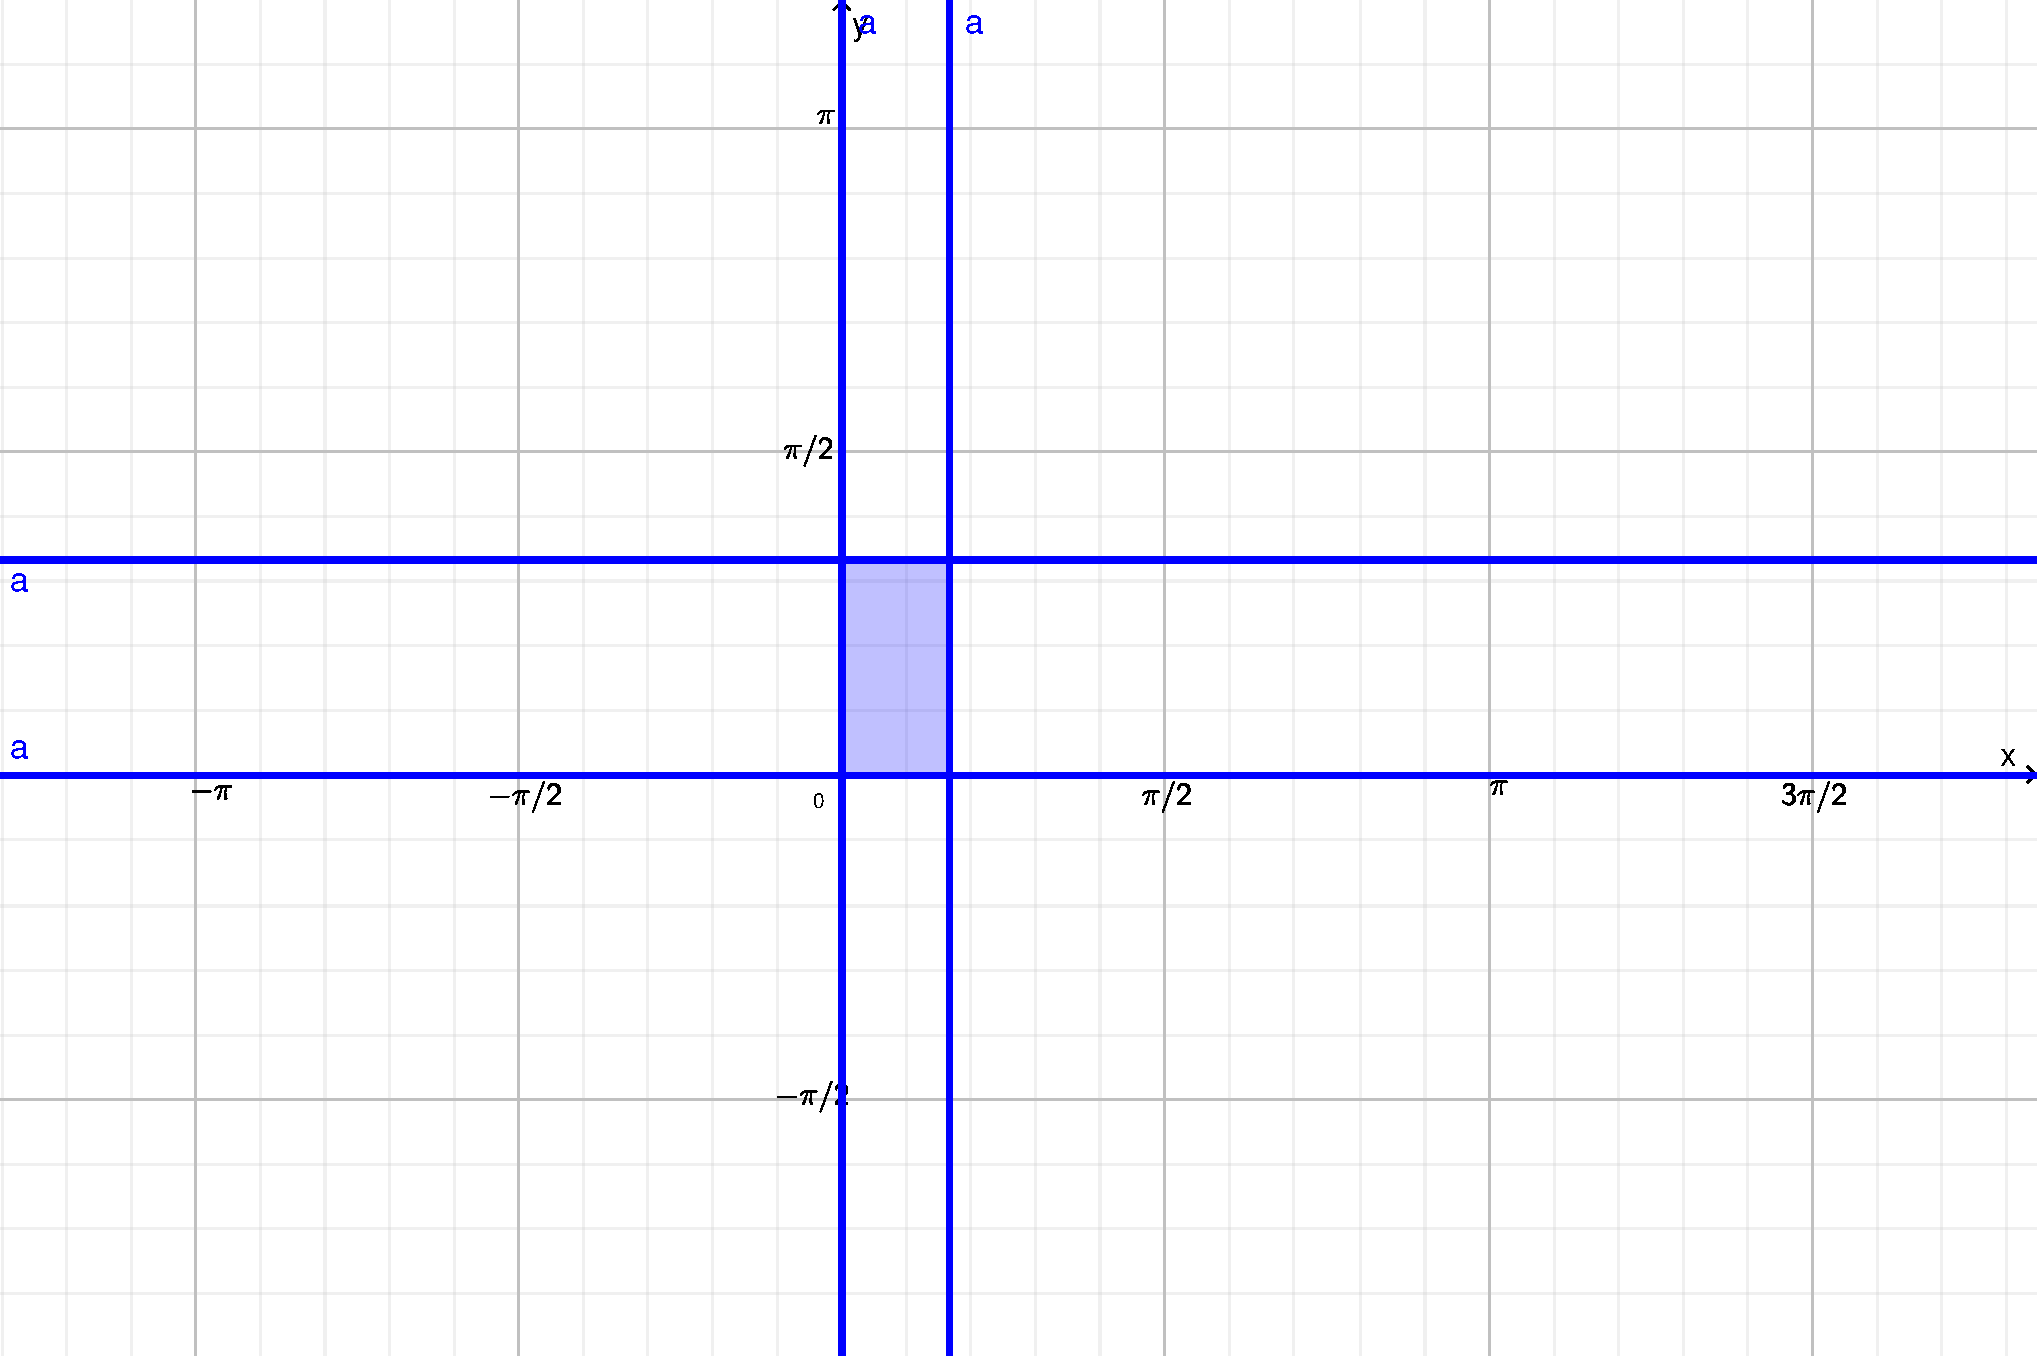
\includegraphics[width=0.7\linewidth]{fig/integrais-multiplas-1a}
		\caption{Região de integração}
		\label{fig:integrais-multiplas-1a}
	\end{figure}
	
	\begin{equation*}
		S = \int_{0}^{\frac{\pi}{6}} \int_{0}^{\frac{\pi}{3}} x \sen (x + y) dy dx
	\end{equation*}
	
	\begin{equation*}
		S = \int_{0}^{\frac{\pi}{6}} \left[ - x \cos (x + y) \right]_{0}^{\frac{\pi}{3}} dx
	\end{equation*}
	
	\begin{equation*}
		S = \int_{0}^{\frac{\pi}{6}} \left[ x \cos (x) - x \cos \left(x + \frac{\pi}{3} \right) \right]_{0}^{\frac{\pi}{3}} dx
	\end{equation*}
	
	\begin{equation*}
		S = \left[ x \sen (x) - \int \sen (x) dx - x \sen \left( x + \frac{\pi}{3} \right) + \int \sen \left( x + \frac{\pi}{3} \right) dx \right]_{0}^{\frac{\pi}{6}}
	\end{equation*}
	
	\begin{equation*}
		S = \left[ x \sen (x) +  \cos (x) - x \sen \left( x + \frac{\pi}{3} \right) - \cos \left( x + \frac{\pi}{3} \right) \right]_{0}^{\frac{\pi}{6}}
	\end{equation*}
	
	\begin{equation*}
		S = \left[ \frac{\pi}{6} \sen \left(\frac{\pi}{6}\right) +  \cos \left(\frac{\pi}{6}\right) - \frac{\pi}{6} \sen \left( \frac{\pi}{6} + \frac{\pi}{3} \right) - \cos \left( \frac{\pi}{6} + \frac{\pi}{3} \right) \right] \\- \left[ 0 \sen (0) +  \cos (0) - 0 \sen \left( 0 + \frac{\pi}{3} \right) - \cos \left( 0 + \frac{\pi}{3} \right) \right]
	\end{equation*}
	
	\begin{equation*}
		S = \left[ \frac{\pi}{6} \frac{1}{2} + \frac{\sqrt{3}}{2} - \frac{\pi}{6} 1 - 0 \right] - \left[ 1 - \frac{1}{2} \right]
	\end{equation*}
	
	\begin{equation*}
	S = \left[ \frac{\pi}{12} + \frac{\sqrt{3}}{2} - \frac{\pi}{6} \right] - \left[ \frac{1}{2} \right]
	\end{equation*}
	
	\begin{equation*}
	S = \left[ \frac{6\sqrt{3} - \pi}{12} \right] - \left[ \frac{1}{2} \right]
	\end{equation*}
	
	\begin{equation*}
		S = \left[ \frac{6\sqrt{3} - \pi}{12} \right] - \left[ \frac{1}{2} \right]
	\end{equation*}
	
	\begin{equation*}
		S = \frac{\sqrt{3}}{2} - \frac{\pi}{2} - \frac{1}{2} \quad unidades\quad de \quad \acute{a}rea
	\end{equation*}
	
	\section*{Questão 2}
	
	Dada a integral tripla $ \int_{0}^{2} \int_{0}^{\frac{y}{2}} \int_{0}^{y-2x} dz dx dy $, desenvolva os seguintes itens.
	
	\begin{enumerate}[a]
		\item Faça a descrição analítica do domínio de integração.
		\item Faça a descrição gráfica da região de integração no plano xy.
		\item Calcule a integral dada. O que o resultado pode significar?
		\item Qual a função que delimita o sólido inferiormente e qual a função que delimita o sólido superiormente?
	\end{enumerate}
	
	(Valor da questão: 1,0)
	
	Descrição analítica do domínio de interação no sistema de inequações \ref{eq:desc_analitic2}.
	
	\begin{equation} \label{eq:desc_analitic2}
		\left\{
			\begin{array}{l}
				0 \le z \le y - 2x \\
				0 \le x \le \frac{y}{2} \\
				0 \le y \le 2
			\end{array}
		\right.
	\end{equation}
	
	A descrição gráfica da região de integração no plano xy é apresentada na figura \ref{fig:integrais-multiplas-2a}
	
	\begin{figure}[h]
		\centering
		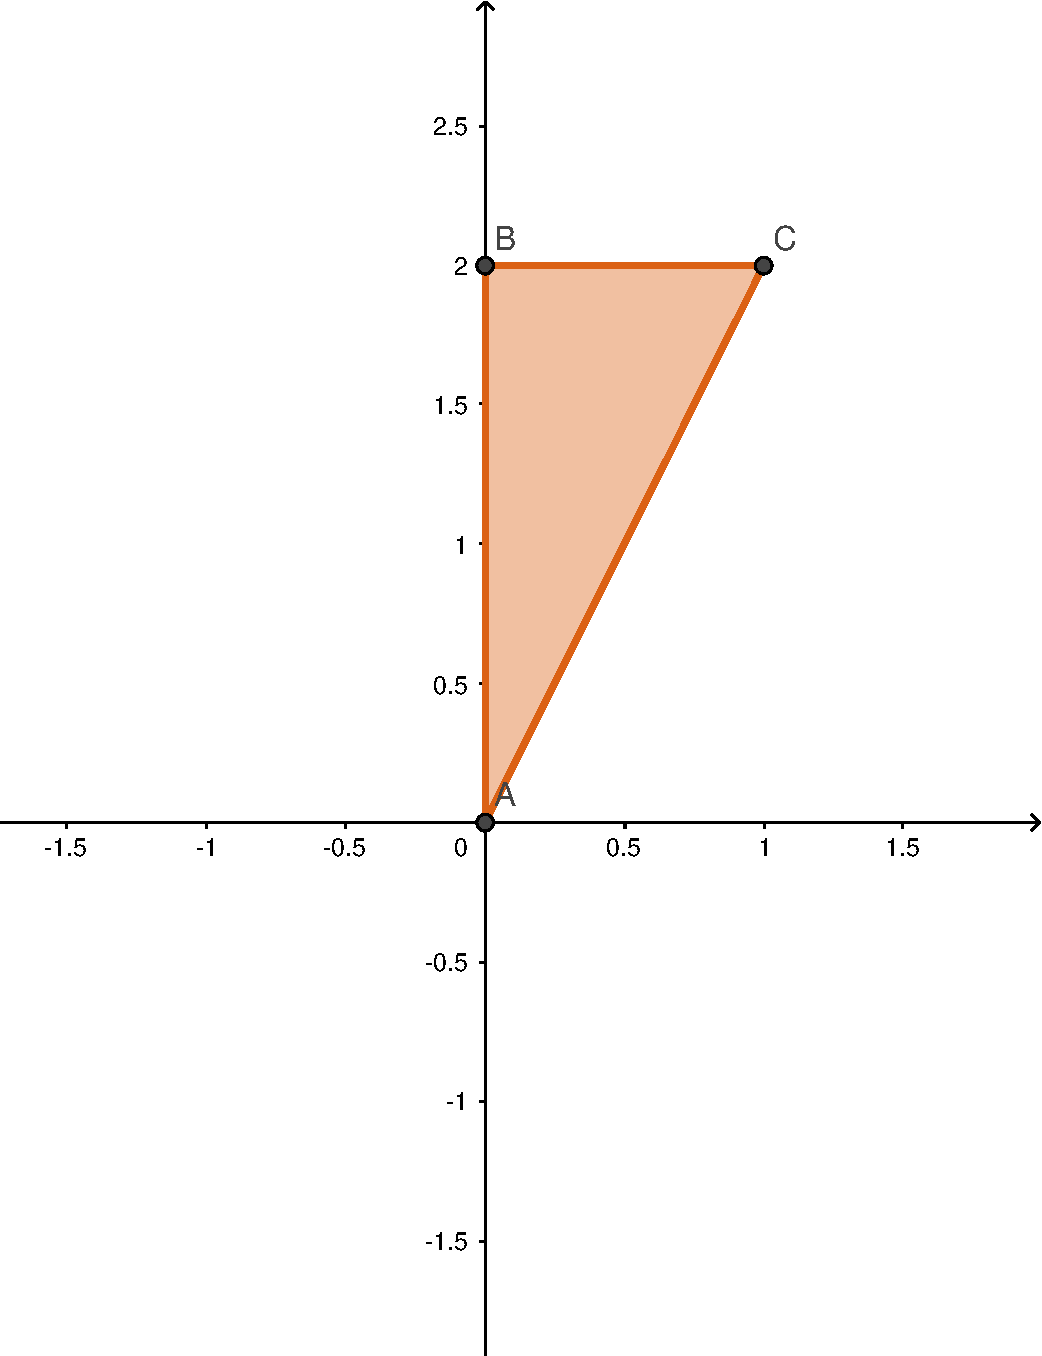
\includegraphics[width=0.7\linewidth]{fig/integrais-multiplas-2a}
		\caption{Domínio de Integração}
		\label{fig:integrais-multiplas-2a}
	\end{figure}
	
	\begin{equation*}
		S = \int_{0}^{2} \int_{0}^{\frac{y}{2}} \int_{0}^{y-2x} dz dx dy
	\end{equation*}
	
	\begin{equation*}
		S = \int_{0}^{2} \int_{0}^{\frac{y}{2}} \left(y-2x \right) dx dy
	\end{equation*}
	
	\begin{equation*}
		S = \int_{0}^{2} \left[ yx-x^2 \right]_0^{\frac{y}{2}} dy
	\end{equation*}

	\begin{equation*}
		S = \int_{0}^{2} \left[ \left(\frac{y^2}{2}-\frac{y^2}{4}\right) - \left(y0-0^2\right) \right] dy
	\end{equation*}	
	
	\begin{equation*}
		S = \int_{0}^{2} \left[\frac{y^2}{2}-\frac{y^2}{4} \right] dy
	\end{equation*}	
	
	\begin{equation*}
		S = \int_{0}^{2} \left[\frac{2y^2}{4}-\frac{y^2}{4} \right] dy
	\end{equation*}
	
	\begin{equation*}
		S = \int_{0}^{2} \left[\frac{y^2}{4}\right] dy
	\end{equation*}	
	
	\begin{equation*}
		S = \left[\frac{y^3}{12} \right]_0^2
	\end{equation*}
	
	\begin{equation*}
		S = \frac{8}{12}
	\end{equation*}
	
	\begin{equation*}
		S = \frac{1}{3} \quad unidades \quad de \quad volume
	\end{equation*}
	
	O resultado pode significar o volume do sólido.
	
	A função que delimita inferiormente o sólido é $ z = 0 $ e superiormente é $ z = y - 2x $
	
	\section*{Questão 3}
	
	Dada a integral $ \int \int_R x e^{xy} dA $, sendo que R é a região dos pontos do plano xy dada pelo produto cartesiano $ R=[0, 1] \times [0, 1] $.
	
	\begin{enumerate}[a]
		\item Fazer a descrição analítica da região de integração.
		\item Fazer a descrição gráfica da região de integração.
		\item Escrever a integral em diferentes ordens de integração
		\item Calcular a integral usando a ordem mais conveniente.
	\end{enumerate}

	(Valor da questão: 1,0)

	Descrição analitica da região de interação no sistema de inequações \ref{eq:desc_analitica3}.
	
	\begin{equation} \label{eq:desc_analitica3}
		\left\{
			\begin{array}{l}
				0 \le y \le 1 \\
				0 \le x \le 1
			\end{array}
		\right.
	\end{equation}
	
	A Descrição grágica da região de integração segue na figura \ref{fig:integrais-multiplas-3a}.
	
	\begin{figure}[h]
		\centering
		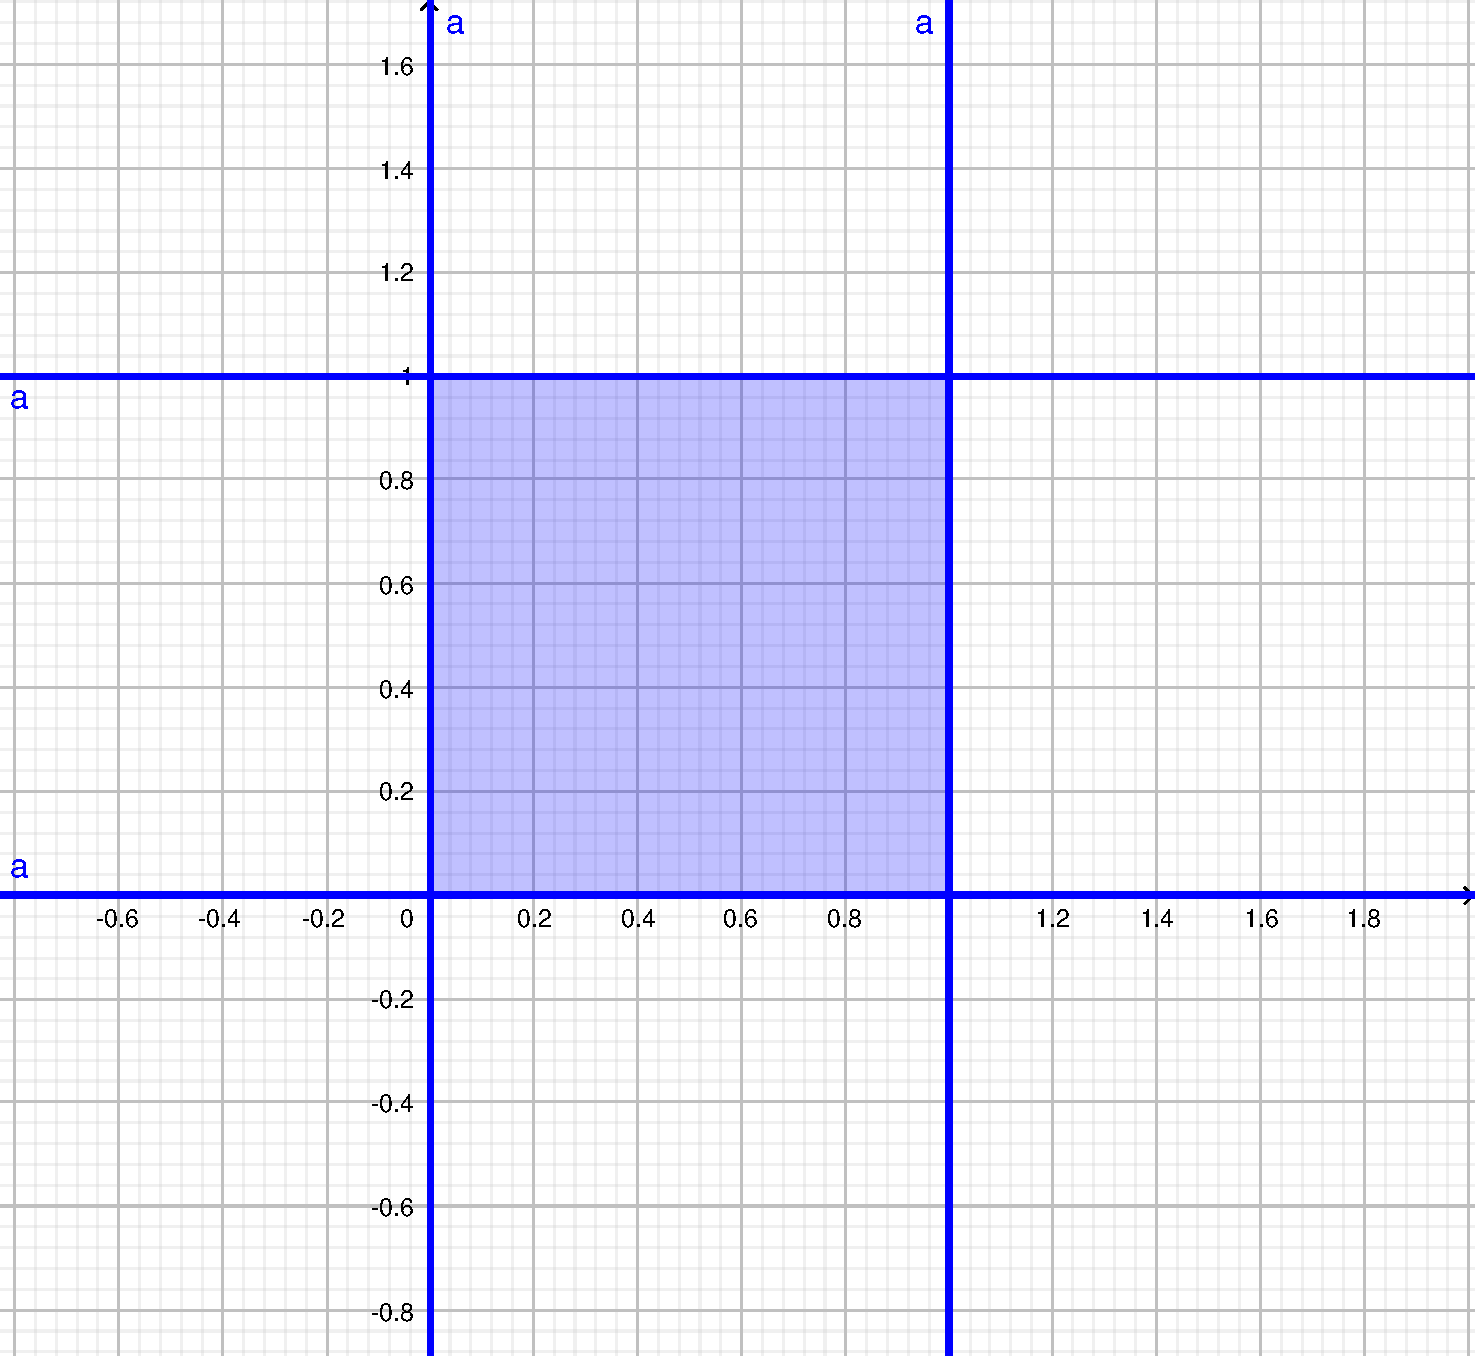
\includegraphics[width=0.7\linewidth]{fig/integrais-multiplas-3a}
		\caption{Descrição gráfica da Região de Integração}
		\label{fig:integrais-multiplas-3a}
	\end{figure}

	Segue a integral escrita em diferentes ordens de integração em \ref{eq:ordemdxdy} e \ref{eq:ordemdydx}.

	\begin{equation} \label{eq:ordemdxdy}
		\int_0^1 \int_0^1 x e^{xy} dx dy
	\end{equation}
	
	\begin{equation} \label{eq:ordemdydx}
		\int_0^1 \int_0^1 x e^{xy} dy dx
	\end{equation}
	
	Parece que a equação \ref{eq:ordemdydx} é a mais conveniente, pois no caso \ref{eq:ordemdxdy}, iniciariamos a primeira integral por partes.
	
	\begin{equation*}
		\int_0^1 \int_0^1 x e^{xy} dy dx
	\end{equation*}
	
	\begin{equation*}
		\int_0^1 \left[ x e^{xy} \right]_0^1 dx
	\end{equation*}
	
	\begin{equation*}
		\int_0^1 \left[ e^x - 1 \right] dx
	\end{equation*}
	
	\begin{equation*}
		\left[ e^x - x\right]_0^1
	\end{equation*}
	
	\begin{equation*}
		e - 1 - 1 + 0
	\end{equation*}
	
	\begin{equation}
		e - 2
	\end{equation}
	
	\section*{Questão 4}
	
	Determinar o volume do sólido delimitado por:
	
	$ z = 2x+3y+4 $
	
	$ x = 0 $
	
	$ x = 1 $
	
	$ y = 0 $
	
	$ y = 2 $
	
	(Valor da Questão: 1.0)
	
	
	
	\begin{equation*}
		R:
		\begin{cases}
			0 \le x \le 1 \\
			0 \le y \le 2 \\
			0 \le 2x + 3y + 4
		\end{cases}
	\end{equation*}
	
	\begin{equation*}
		\int_{0}^{1} \int_{0}^{2} \int_{0}^{2x + 3y + 4} dz dy dx
	\end{equation*}
	
	\begin{equation*}
		\int_{0}^{1} \int_{0}^{2} 2x + 3y + 4 dy dx
	\end{equation*}
	
	\begin{equation*}
		\int_{0}^{1} \left[2xy + \frac{3}{2}y^2 + 4y\right]_{0}^{2} dx
	\end{equation*}
	
	\begin{equation*}
		\int_{0}^{1} \left[4x + 6 + 8\right] dx
	\end{equation*}
	
	\begin{equation*}
		\int_{0}^{1} \left[4x + 14\right] dx
	\end{equation*}
	
	\begin{equation*}
		\left[2x^2 + 14x\right]_{0}^{1}
	\end{equation*}
	
	\begin{equation}
		16
	\end{equation}
	
	\section*{Questão 5}
	
	Calcule a integral dupla $ \int \int_R \exp{\frac{y}{x}} dA $, sendo R a região dada por:
	
	$ y = x^3 $
	
	$ y = x $
	
	$ 1 \le x \le 2 $
	
	O cálculo obtido representa a área da região R? Justifique a sua resposta
	
	(Valor da questão: 1,0)
	
	\begin{equation*}
		R: 
		\begin{cases}
			1 \le x \le 2\\
			x \le y \le x^3
		\end{cases}
	\end{equation*}
	
	\begin{equation*}
		\int_{1}^{2} \int_{x}^{x^3} e^{\frac{y}{x}} dy dx
	\end{equation*}
	
	\begin{equation*}
		\int_{1}^{2} \left[ x e^{\frac{y}{x}} \right]_{x}^{x^3} dx
	\end{equation*}
	
	\begin{equation*}
		\int_{1}^{2} \left[ x e^{x^2} - x e \right] dx
	\end{equation*}
	
	\begin{equation*}
		\left[ \frac{1}{2}e^{x^2} - \frac{1}{2}x^2 e \right]_1^2
	\end{equation*}
	
	\begin{equation*}
		\frac{1}{2}e^{2^2} - \frac{1}{2}2^2 e - \frac{1}{2}e^{1^2} + \frac{1}{2}1^2 e
	\end{equation*}
	
	\begin{equation*}
		\frac{1}{2}e^4 - 2 e - \frac{1}{2}e + \frac{1}{2} e
	\end{equation*}
	
	\begin{equation*}
		\frac{1}{2}e^4 - 2 e
	\end{equation*}
	
	\section*{Questão 6}
	
	Usando integrais triplas, calcule o volume do sólido acima da superfície $ z = x^2 + y^2 $ e abaixo da superfície $ z = 4 - x^2 - y^2 $.
	
	(Valor da questão: 1,0)
	
	Encontrando a intersecção entre as duas superfícies.
	
	\begin{equation*}
		x^2 + y^2 = 4 - x^2 - y^2
	\end{equation*}
	
	\begin{equation*}
		2x^2 + 2y^2 = 4
	\end{equation*}
	
	\begin{equation*}
		x^2 + y^2 = 2
	\end{equation*}
	
	A região de integração está escrita em \ref{eq:regiao6carteziana}.
	
	\begin{equation}\label{eq:regiao6carteziana}
		R:
		\begin{cases}
			x^2 + y^2 \le z \le 4 - x^2 - y^2\\
			-\sqrt{2 - x^2} \le y \le \sqrt{2 - x^2}\\
			-\sqrt{2} \le x \le \sqrt{2}
		\end{cases}
	\end{equation}
	
	Ou ainda em coordenadas cilíndricas conforme \ref{eq:regiao6cilindricas}.
	\begin{equation}\label{eq:regiao6cilindricas}
		R':
		\begin{cases}
			r^2 \le z \le 4 - r^2\\
			0 \le r \le \sqrt{2}\\
			0 \le \theta \le 2\pi
		\end{cases}
	\end{equation}
	
	\begin{equation*}
		V = \int_{0}^{2\pi} \int_{0}^{\sqrt{2}} \int_{r^2}^{4 - r^2} r dz dr d\theta
	\end{equation*}
	
	\begin{equation*}
		V = \int_{0}^{2\pi} \int_{0}^{\sqrt{2}} (4 - 2r^2)r dr d\theta
	\end{equation*}
	
	\begin{equation*}
		V = \int_{0}^{2\pi} \int_{0}^{\sqrt{2}} 4r - 2r^3 dr d\theta
	\end{equation*}
	
	\begin{equation*}
		V = \int_{0}^{2\pi} \left[2r^2 - \frac{1}{2}r^4\right]_0^{\sqrt{2}} d\theta
	\end{equation*}
	
	\begin{equation*}
		V = \int_{0}^{2\pi} 2 d\theta
	\end{equation*}

	\begin{equation*}
		V = \left[2 \theta\right]_0^{2\pi}
	\end{equation*}
	
	\begin{equation*}
		V = 4\pi
	\end{equation*}

	\section*{Questão 7}
	
	Calcule a seguinte integral usando coordenadas esféricas:
	
	$ \int \int \int_R (x^2 + y^2 + z^2)^2 dV $, sendo que B é a bola com sentro na origem e raio 4.
	
	A região B está algebrizada em \ref{eq:B7}
	\begin{equation}\label{eq:B7}
		B:
		\begin{cases}
		0 \le \rho \le 4\\
		0 \le \phi \le \pi \\
		0 \le \theta \le 2\pi
		\end{cases}
	\end{equation}
	
	\begin{equation*}
		M = \int_{0}^{2\pi} \int_{0}^{\pi} \int_{0}^{4} (\rho^2)^2 \rho^2 \sen \phi d\rho d\phi d\theta
	\end{equation*}
	
	\begin{equation*}
		M = \int_{0}^{2\pi} \int_{0}^{\pi} \int_{0}^{4} \rho^6 \sen \phi d\rho d\phi d\theta
	\end{equation*}
	
	\begin{equation*}
		M = \int_{0}^{2\pi} \int_{0}^{\pi} \left[ \frac{1}{7}\rho^7 \sen \phi \right]_{0}^{4} d\phi d\theta
	\end{equation*}
	
	\begin{equation*}
		M = \int_{0}^{2\pi} \int_{0}^{\pi} \frac{1}{7}4^7 \sen \phi  d\phi d\theta
	\end{equation*}
	
	\begin{equation*}
		M = \frac{1}{7}4^7 \int_{0}^{2\pi} \int_{0}^{\pi} \sen \phi  d\phi d\theta
	\end{equation*}
	
	\begin{equation*}
		M = \frac{1}{7}4^7 \int_{0}^{2\pi} \left[-\cos \phi\right]_0^{\pi}  d\theta
	\end{equation*}
	
	\begin{equation*}
		M = \frac{1}{7}4^7 \int_{0}^{2\pi} 2 d\theta
	\end{equation*}
	
	\begin{equation*}
		M = \frac{2}{7}4^7 \int_{0}^{2\pi} d\theta
	\end{equation*}
	
	\begin{equation*}
		M = \frac{2}{7}4^7 \cdot 2\pi
	\end{equation*}
	
	\begin{equation*}
		M = \frac{4^8}{7}\pi
	\end{equation*}
	
	\begin{equation*}
		M = \frac{65536}{7}\pi
	\end{equation*}
	
	\section*{Questão 8}
	
	Calcule $ \int_{0}^3 \int_{0}^{\sqrt{9-y^2}} \int_{\sqrt{x^2+y^2}}^{\sqrt{18-x^2-y^2}} (x^2 + y^2 + z^2) dz dx dy $. Use coordenadas esféricas. O resultado obtido representa um volume? Justifique a sua resposta.
	
	(Valor da questão: 1,0)
	
	\begin{equation}
		B:
		\begin{cases}
		0 \le \rho \le 3\sqrt{2}\\
		0 \le \phi \le \frac{\pi}{4}\\
		0 \le \theta \le 2\pi
		\end{cases}
	\end{equation}
	
	\begin{equation}
		\int_{0}^{2\pi} \int_{0}^{\frac{\pi}{4}} \int_{0}^{3\sqrt{2}} r^2 r^2 \sen \phi d\rho d\phi d\theta
	\end{equation}
	
	\begin{equation}
		\int_{0}^{2\pi} \int_{0}^{\frac{\pi}{4}} \left[ \frac{1}{5}r^5 \sen \phi \right]_{0}^{3\sqrt{2}} d\phi d\theta
	\end{equation}
	
	\begin{equation}
		\int_{0}^{2\pi} \int_{0}^{\frac{\pi}{4}} \frac{972\sqrt{2}}{5} \sen \phi d\phi d\theta
	\end{equation}
	
	\begin{equation}
		\int_{0}^{2\pi} \left[-\frac{972\sqrt{2}}{5} \cos \phi \right]_{0}^{\frac{\pi}{4}} d\theta
	\end{equation}
	
	\begin{equation}
		\int_{0}^{2\pi} \left(-\frac{972\sqrt{2}}{5} \cos \frac{\pi}{4} + \frac{972\sqrt{2}}{5} \cos 0 \right) d\theta
	\end{equation}
	
	\begin{equation}
		\int_{0}^{2\pi} \left(-\frac{972\sqrt{2}}{5} \frac{\sqrt{2}}{2} + \frac{972\sqrt{2}}{5} \right) d\theta
	\end{equation}
	
	\begin{equation}
		\int_{0}^{2\pi} \left(-\frac{972}{5} + \frac{972\sqrt{2}}{5} \right) d\theta
	\end{equation}
	
	\begin{equation*}
		\int_{0}^{2\pi} \frac{972(\sqrt{2} - 1)}{5} d\theta
	\end{equation*}
	
	\begin{equation*}
		\frac{972(\sqrt{2} - 1)}{5} 2\pi
	\end{equation*}
	
	\begin{equation*}
		\frac{1944\pi(\sqrt{2} - 1)}{5}
	\end{equation*}
	
	O resultado não representa um volume pois a função sendo integrada é diferente de 1.
	
	
	\section*{Questão 9}
	
	Escolha algumas funções e tente fazer a modelagem de um sólido usando um software livre a sua esoclha. O sólido não deve ter o volume encontrado por fórmulas da Geometria. Relate aqui nessa questão essa sua experiência e apresente as funções escolindas e o sólido montado no software. Caso você pesquise em livros ou na internet, apresente aqui a referência bibliográfica.
	
	(Valor da questão: 1,0)
	
	\section*{Questão 10}
	
	Relate aqui sua participação nos Fóruns 1 e 2.
\end{document}